\documentclass[11pt,a4paper]{article}
\usepackage[utf8]{inputenc}
\usepackage[T1]{fontenc}
\usepackage{babel}
\babelprovide[main,import]{polish}
\usepackage{lmodern,amsmath,booktabs,microtype}
\usepackage[margin=27mm]{geometry}
\usepackage{tikz}
\usetikzlibrary{positioning,arrows.meta,babel}
\usepackage[round,authoryear]{natbib}
\usepackage[hidelinks]{hyperref}
\title{Eksperymentalne odróżnianie motywów ponoszenia osobistego kosztu}
\author{Mateusz Pomianek}
\date{MSC-PAIN-P07 \enspace PROSPECTIVE \enspace wersja 1.0.0 \enspace 26.11.2026}
\setlength{\emergencystretch}{3em}
\begin{document}
\maketitle
\begin{abstract}
Przedstawiono projekt eksperymentu online, w którym uczestnik rozstrzyga, czy zaakceptować osobisty koszt w zamian za korzyść anonimowego odbiorcy. Niezależnie zmieniają się koszt, widoczność indywidualnej decyzji i wielkość korzyści odbiorcy. Głównym estymandem jest interakcja kosztu i widoczności na skali warunkowego logarytmu szans. Wzorzec wyborów pozwoli ocenić konkurencyjne przewidywania dotyczące wartości skutku dla odbiorcy i wartości społecznej czynu. Empatia, oczekiwana ocena oraz uwewnętrznione normy pozostają możliwymi wyjaśnieniami. Liczebność planuje się z użyciem symulacji Monte Carlo. Projekt nie obejmuje akwizycji danych neuronalnych ani uzyskanych wyników empirycznych.
\end{abstract}

\section{Ramy teoretyczne}
Ta sama decyzja może mieć kilka źródeł. Troska o rezultat dla odbiorcy przewiduje większą częstotliwość pomocy przy większej korzyści dla odbiorcy, również przy wyborze prywatnym. Model nieczystego altruizmu dopuszcza niezależną wartość samego udzielenia pomocy \citep{andreoni1990}. Pozytywna reakcja na akt pomocy może współistnieć z troską o odbiorcę. Badania nad empatią i możliwością opuszczenia sytuacji wskazują, jak rozdzielać przewidywania dotyczące troski o drugą osobę i redukcji własnego dyskomfortu \citep{batson1981}. P07 utrzymuje opis odbiorcy i jego potrzebę na stałym poziomie. Korzyść odbiorcy określa skuteczność działania, a empatia nie jest manipulowana.

Widoczność umożliwia ocenę społeczną wykonawcy. Model reputacji i obrazu siebie dopuszcza, że ten sam czyn niesie informację o preferencjach decydenta \citep{benabou2006}. Badania nad motywacją wizerunkową wykorzystują różnicę między działaniem widocznym a prywatnym \citep{ariely2009}. Metaanaliza wskazuje na zależność związku obserwowalności i prospołeczności od kontekstu \citep{bradley2018}. Przy wyborze partnera publiczna hojność może funkcjonować jako sygnał skłonności do współpracy \citep{barclay2007}. P07 bada słabsze przewidywanie: obserwator zna wymagany koszt, więc widoczność może podnosić atrakcyjność kosztownych decyzji silniej niż atrakcyjność decyzji tanich. Obserwator nie wybiera później partnera i nie przyznaje wypłaty. Test dotyczy zatem sygnalizacji ocenianej przez odbiorcę sygnału, bez testowania opłacalności w równowadze sygnalizacyjnej.

Zgodność z normą może zwiększać pomoc prywatną, a oczekiwanie sankcji lub aprobaty może zmieniać wybory publiczne. Oceny stosowności przewidują decyzje w wariantach gry dyktatora \citep{krupka2013}. Manipulacja przejrzystością konsekwencji pokazuje, że interpretacja hojnego wyboru zależy także od możliwości usprawiedliwienia decyzji \citep{dana2007}. Niepewna skuteczność może też służyć usprawiedliwianiu odmowy przy konflikcie interesów \citep{exley2016}. W P07 konsekwencje są jawne w obu warunkach widoczności. Wzrost pomocy w sytuacji publicznej pozostaje zgodny zarówno z poszukiwaniem aprobaty, jak i z unikaniem potępienia. Wzrost pomocy wraz z korzyścią prywatną dla odbiorcy jest zgodny także z normą skutecznej pomocy.

\subsection{Wartość decyzji}
Różnicę użyteczności między podjęciem działania a odmową można zapisać jako
\[
\Delta U_i=-a_i c+b_i g+w_i+n_i(c,g,v)+v\,r_i(c,g)+\varepsilon_i,
\]
gdzie $c$ oznacza koszt decydenta, $g$ oznacza korzyść odbiorcy, a $v=1$ oznacza widoczność. Współczynniki $a_i$ i $b_i$ opisują wrażliwość na koszt i korzyść. Składnik $w_i$ określa wartość aktu pomocy, $n_i$ zgodność z normą, a $r_i$ wartość oczekiwanej oceny. O dodatnim H1 może decydować wzrost $r_i$ wraz z kosztem, ale także zależność $n_i$ od kosztu i widoczności. Empatia może zwiększać $b_i$ lub $w_i$. Przy ośmiu warunkach i jednym wskaźniku wyboru nie da się oddzielnie oszacować wszystkich tych wielkości. GLMM estymuje kontrasty behawioralne wynikające z randomizacji.

\subsection{Kontekst neuropsychologiczny}
W eksperymencie fMRI dotyczącym darowizn sygnał w brzuszno-przyśrodkowej korze przedczołowej wiązał się z subiektywną wartością darowizny. Autorzy analizowali też łączność funkcjonalną z obszarami związanymi z poznaniem społecznym \citep{hare2010}. Daje to podstawę do hipotezy o integracji informacji dotyczących siebie i innych podczas wyboru. Dane P07 będą obejmowały decyzje i odpowiedzi na pytania kontrolne. Estymowane kontrasty opiszą skutki warunków zadania na poziomie zachowania.

\begin{figure}[htbp]
\centering
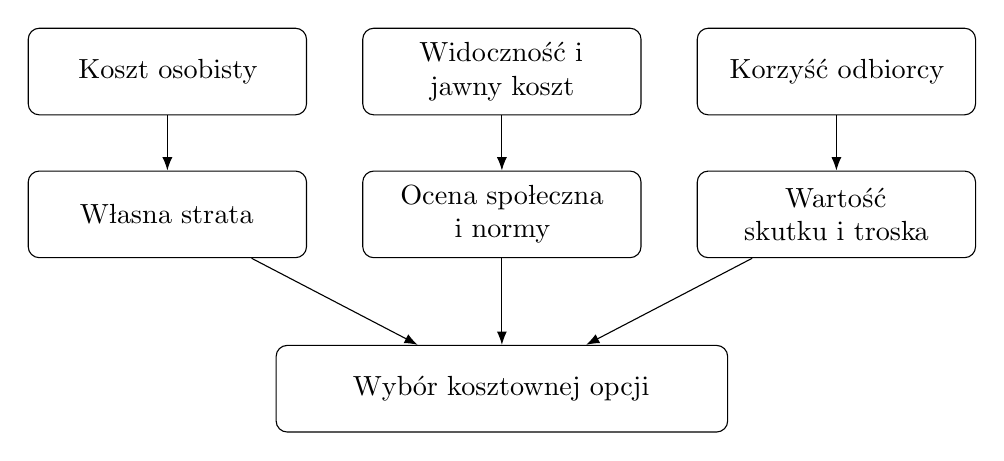
\begin{tikzpicture}[box/.style={draw,rounded corners,align=center,text width=33mm,minimum height=11mm},>=Latex]
\node[box] (c) {Koszt osobisty};
\node[box,right=7mm of c] (v) {Widoczność i jawny koszt};
\node[box,right=7mm of v] (b) {Korzyść odbiorcy};
\node[box,below=7mm of c] (s) {Własna strata};
\node[box,below=7mm of v] (r) {Ocena społeczna i normy};
\node[box,below=7mm of b] (o) {Wartość skutku i troska};
\node[box,below=11mm of r,text width=55mm] (y) {Wybór kosztownej opcji};
\draw[->] (c)--(s); \draw[->] (v)--(r); \draw[->] (b)--(o);
\draw[->] (s)--(y); \draw[->] (r)--(y); \draw[->] (o)--(y);
\end{tikzpicture}
\caption{Konkurencyjne drogi wpływu warunków wyboru. Wartość samego aktu pomocy i uwewnętrzniona norma mogą działać w obu warunkach widoczności. Mechanizmy pośredniczące pozostają hipotezami.}
\end{figure}

\section{Pytania i hipotezy}
Czy obserwacja osłabia spadek gotowości do pomocy przy wzroście kosztu? Czy pomoc prywatna reaguje na korzyść odbiorcy? Czy koszt ogranicza gotowość do pomocy uśrednioną po pozostałych warunkach?
\begin{description}
\item[H1.] Różnica publiczny kontra prywatny w warunkowych logarytmach szans wyboru pomocy jest większa przy wysokim niż przy niskim koszcie, po równym uśrednieniu kontrastu po poziomach korzyści.
\item[H2.] W warunku prywatnym większa korzyść odbiorcy zwiększa warunkowy logarytm szans wyboru pomocy, po równym uśrednieniu po poziomach kosztu.
\item[H3.] Wyższy koszt obniża warunkowy logarytm szans wyboru pomocy po równym uśrednieniu po poziomach korzyści i widoczności.
\end{description}
Efekt w kierunku przeciwnym podważy dane przewidywanie. Nieprecyzyjny przedział przecinający zero pozostawi pytanie nierozstrzygnięte. Efekty H1 i H2 mogą współwystępować. H1 jest warunkiem przewidywanego wzorca kosztownej sygnalizacji, lecz oczekiwana aprobata dla wyrzeczenia lub popyt eksperymentalny mogą dawać ten sam wzorzec. H2 podważa opis oparty wyłącznie na stałej wartości aktu pomocy przy stałym koszcie, jeśli pozostałe determinanty są stałe. Rozdzielenie empatii, normy i korzyści dla obrazu siebie wymagałoby dodatkowych manipulacji.

\section{Zakres i nowość}
MSC-PAIN-P02 zakłada pomiar lęku przed szczęściem i przyszłością oraz analizę jego związku z unikaniem kosztu, z uwzględnieniem wspólnej wariancji negatywnego afektu. P07 szacuje kontrasty przyczynowe w obrębie osoby na podstawie losowej kolejności warunków i jawnie rozdzielonych skutków dla decydenta i odbiorcy. Brak wspólnego głównego predyktora, estymandu i planu danych. Porównanie odnosi się do jawnych szkiców ARC Neuro. Odrębność wobec pełnego protokołu źródłowego P02 pozostaje do potwierdzenia.

Wkład względem literatury polega na wspólnym teście w tym samym zadaniu, z osobnymi osiami kosztu i korzyści oraz obserwatorem bez prawa do rewanżu. Literatura obejmuje już manipulacje widocznością, wybór partnera, efektywność pomocy i ocenę norm. Przegląd ukierunkowany nie ustanawia pierwszeństwa. W niniejszym projekcie o jego wartości informuje zdolność oszacowania interakcji kosztu i widoczności przy stałej korzyści odbiorcy.

\section{Eksperyment online}
Schemat wewnątrzosobniczy $2\times2\times2$ obejmuje 24 próby, po trzy na kombinację. Decyzja ma dwie opcje. A zachowuje 6 zł bonusu decydenta i nie dodaje bonusu odbiorcy. B pomniejsza bonus decydenta o 1 lub 4 zł oraz zwiększa bonus anonimowego odbiorcy o 2 lub 5 zł, z niezależnego budżetu. Odbiorca nie zna decyzji ani tożsamości decydenta. Prywatność oznacza brak ujawnienia decyzji obserwatorowi. W warunku widocznym niezależny obserwator otrzymuje jednorazowy kod, obydwie opcje i decyzję w jednej wylosowanej do realizacji próbie. Widzi również odmowę, jeżeli wybrano A. Dane badawcze są pseudonimizowane w obu warunkach. Obserwator nie kontaktuje się z decydentem.

Kolejność 24 prób losuje się jednolicie z wielozbioru kombinacji, niezależnie dla każdej osoby. Pozycję opcji równoważy się losowo między osobami. Po zakończeniu losuje się jedną z 24 prób z równymi szansami do realizacji. Kwoty nie kumulują się. Dzięki temu widoczność i koszt jednej decyzji nie zmieniają budżetu pozostałych prób. Możliwe pozostają efekty porównywania warunków, przeniesienia i uczenia się. Instrukcje są neutralne i identyczne poza informacją o skutkach oraz ujawnieniu decyzji. Przed zadaniem badany przechodzi sprawdzian rozumienia reguł bez presji czasu. Po nim ocenia wiarygodność ujawnienia, oczekiwaną aprobatę i stosowność, bez wpływu na wypłatę. Oceny są wskaźnikami pomocniczymi bez deklarowanej trafności psychometrycznej.

\begin{figure}[htbp]
\centering
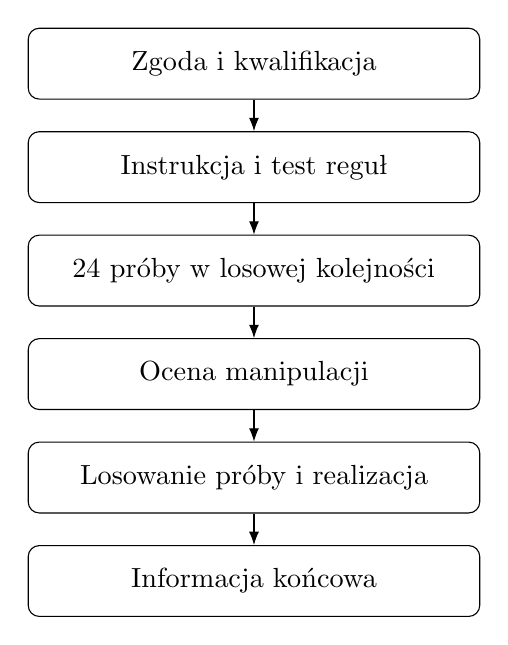
\begin{tikzpicture}[box/.style={draw,rounded corners,align=center,text width=55mm,minimum height=9mm},>=Latex,node distance=4mm]
\node[box] (a) {Zgoda i kwalifikacja};
\node[box,below=of a] (b) {Instrukcja i test reguł};
\node[box,below=of b] (c) {24 próby w losowej kolejności};
\node[box,below=of c] (d) {Ocena manipulacji};
\node[box,below=of d] (e) {Losowanie próby i realizacja};
\node[box,below=of e] (f) {Informacja końcowa};
\draw[->] (a)--(b); \draw[->] (b)--(c); \draw[->] (c)--(d);
\draw[->] (d)--(e); \draw[->] (e)--(f);
\end{tikzpicture}
\caption{Przebieg projektowanego badania w wariancie z realnymi wypłatami.}
\end{figure}

Wariant hipotetyczny umożliwia bezpłatne sprawdzenie rozumienia zadania i użyteczności interfejsu. Daje estymand dla deklarowanych wyborów w opisie sytuacji. Hipotetyczny koszt i hipotetyczna ocena mogą zmniejszać stawkę decyzji w różnym stopniu, więc kierunku zmiany interakcji H1 nie można ustalić z góry. Wariant rozstrzygający dotyczy rzeczywistych konsekwencji finansowych i ujawnienia. Wymaga zabezpieczenia do 10 zł na decydenta i odbiorcę łącznie, osobno wynagrodzenia za udział, kosztów obserwatorów i obsługi płatności. Dla 320 decydentów górny limit bonusów wynosi 3200 zł, a dla 640 wynosi 6400 zł. Brak finansowania odracza ten wariant. Możliwość wykonania zdalnego wymaga testu przypisania pseudonimów, logowania losowań i realizacji wypłat.

\section{Plan analizy}
Jednostką obserwacji jest próba, jednostką klastrowania osoba. Wynik $Y_{it}=1$ oznacza wybór B. Czynniki $C,V,B$ przyjmują wartości $-0{,}5$ i $+0{,}5$, gdzie dodatni poziom oznacza wyższy koszt, widoczność lub większą korzyść. Model ma pełną strukturę czynnikową:
\begin{align*}
Y_{it}\mid u_i&\sim \operatorname{Bernoulli}(p_{it}), \qquad u_i\sim N(0,\sigma^2),\\
\operatorname{logit}(p_{it})&=\beta_0+u_i+\beta_C C+\beta_V V+\beta_B B\\
&\quad+\beta_{CV}CV+\beta_{CB}CB+\beta_{VB}VB+\beta_{CVB}CVB .
\end{align*}
Główny kontrast H1 to $\beta_{CV}>0$. Kontrasty H2 i H3 to odpowiednio $\beta_B-\beta_{VB}/2>0$ i $\beta_C<0$. Przyjmujemy dwustronny test Walda $\alpha=0{,}05$ i wymagamy zgodnego znaku. Dwa wtórne testy tworzą osobną rodzinę Holma. Pozostałe interakcje i standaryzowane predykcje prawdopodobieństw są opisowe. Raport obejmuje estymaty, 95\% przedziały i osiem prawdopodobieństw wyboru po scałkowaniu po rozkładzie efektu losowego. Iloraz ilorazów szans $\exp(\beta_{CV})$ jest warunkowy. Nie można go utożsamić z różnicą różnic prawdopodobieństw.

Do analizy wchodzą dostępne decyzje po randomizacji. Nieukończona próba ma brak wyniku. Oceny manipulacji i czas odpowiedzi nie służą do wykluczania uczestników. Braki mogą zależeć od trudności wyboru lub widoczności, dlatego podstawowe wnioskowanie zależy od zasadności założenia o ignorowalności braków. Protokół określa analizę wzorców rezygnacji, analizę alternatywnej struktury efektów losowych, model odporny na korelację wewnątrzosobniczą i skrajne imputacje ustalone według znaku kontrastu.

\section{Planowanie liczebności i granice wnioskowania}
Kod Python generuje syntetyczne decyzje, stosuje ten sam model logitowy z losowym wyrazem wolnym i sprawdza dodatni wynik H1. Poziomy efektu 0{,}25, 0{,}40 i 0{,}60 na skali logarytmu ilorazu ilorazów szans stanowią scenariusze projektowe. Scenariusz zerowy kontroluje błąd dodatniego rozstrzygnięcia. Scenariusz heterogeniczny uwzględnia losową wrażliwość na koszt i zwiększony odsetek rezygnacji. Liczebność oznacza uczestników randomizowanych. Zasada wyboru próby wymaga dolnej granicy 95\% przedziału Monte Carlo co najmniej 0{,}80. Nieudane dopasowania zalicza się jako brak rozstrzygnięcia. Wyniki liczbowe zawiera tabela wygenerowana z symulacji.
\begin{table}[htbp]\centering
\caption{Syntetyczna moc dla H1. Najmniejsze $N$ w badanej siatce spełniające kryterium.}
\begin{tabular}{lrrr}\toprule
Scenariusz & $N$ & Moc & 95\% przedział MC \\ \midrule
Mały & 640 & $0{,}920$ & $[0{,}884;\ 0{,}946]$ \\
Umiarkowany & 320 & $0{,}963$ & $[0{,}936;\ 0{,}979]$ \\
Duży & 160 & $0{,}977$ & $[0{,}953;\ 0{,}989]$ \\
Heterogeniczny & 320 & $0{,}937$ & $[0{,}903;\ 0{,}959]$ \\
\bottomrule\end{tabular}\end{table}


Poziom korzyści może sygnalizować także społeczną stosowność wyboru. Osoby mogą traktować widoczność wobec jednego obserwatora inaczej niż publiczność złożoną ze znajomych. Wybór beneficjenta, rozkład dochodu, poziomy kwot i wiarygodność instrukcji ograniczają uogólnianie. Pilotaż wykonalności ma sprawdzić te elementy przed zamrożeniem protokołu. Stan projektu pozostaje \texttt{PROSPECTIVE}. Nie przeprowadzono rekrutacji ani pomiarów w ramach tej wersji.
\bibliographystyle{abbrvnat}
\bibliography{references}
\end{document}
